\documentclass[a4paper]{article}
\usepackage[14pt]{extsizes}

\usepackage[T2A]{fontenc}
\usepackage[utf8]{inputenc}
\usepackage[warn]{mathtext}
\usepackage[russian]{babel}
\usepackage{setspace,amsmath}
\usepackage{graphicx}
\usepackage{epigraph} 
\usepackage{csquotes} 
\usepackage[unicode, pdftex]{hyperref} 
\usepackage{amssymb} 
\usepackage{caption}
\usepackage{amsthm} 
\usepackage{wrapfig}
\usepackage[left=15mm, top=10mm, right=10mm, bottom=15mm, nohead, footskip=10mm]{geometry} 
\RequirePackage{caption}
\DeclareCaptionLabelSeparator{d}{}
\captionsetup{justification=centering,labelsep=d}
\usepackage{multirow}

\begin{document}
\title{\textbf{Лабораторная работа 2.3.1}

\

Получение и измерение вакуума

}
\author{И. Артёмов, Д. Лежнев}
\date{\today}
\maketitle
\noindent

\section*{1. Введение}
	\noindent\textbf{Цель работы:} 1) измерение объемов форвакуумной и высоковакуумной частей установки; 2) определение скорости откачки системы в стационарном режиме, а также по ухудшению и улучшению вакуума.
	
\noindent\textbf{Оборудование:} вакуумная установка с манометрами: масляным, термопарным и ионизационным.
	
\section*{2. Экспериментальна установка}
	
\begin{figure}[h!]
	\centering
	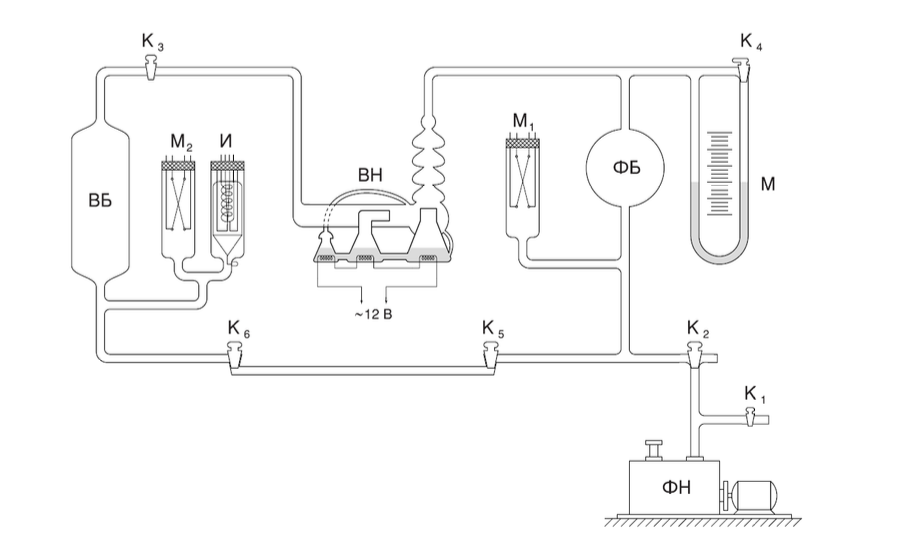
\includegraphics[scale=0.53]{facility.jpg}
	\caption{. Схема экспериментальной установки}
	\label{facility}
\end{figure}

Установка изготовлена из стекла, и состоит из форвакуумного баллона (ФБ), высоковакуумного диффузионного насоса (ВН), высоковакуумного баллона (ВБ), масляного (М) и ионизационного (И) манометров, термопарных манометров ($\text{М}_1$ и $\text{М}_2$), форвакуумного насоса (ФН) и соединительных кранов ($\text{K}_1, \text{K}_2,\; \ldots \;\text{K}_6$) (Рис. \ref{facility}). Кроме того, в состав установки входят: реостат и амперметр для регулирования тока нагревателя диффузионного насоса.
	
\begin{figure}{l}
		\centering
		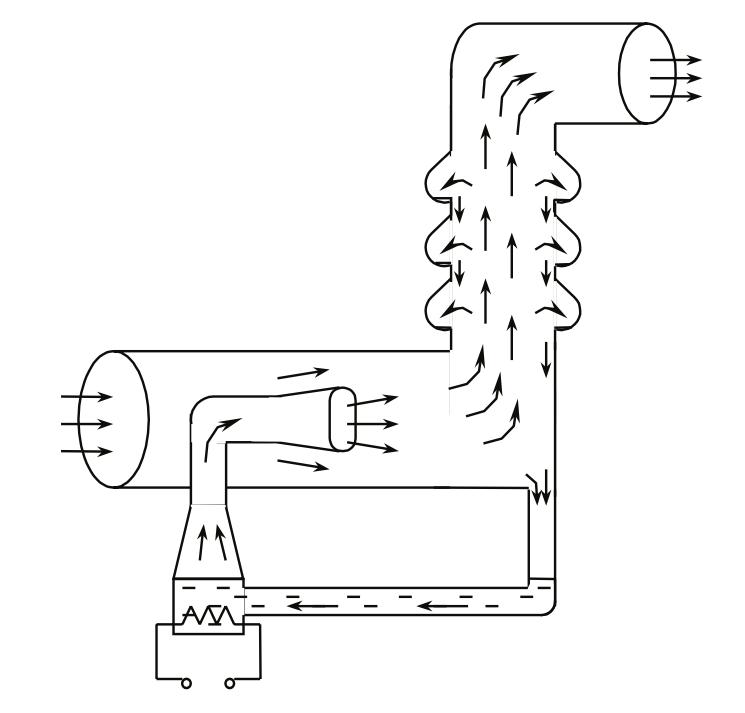
\includegraphics[scale=0.4]{pump.jpg}
		\caption{. Схема работы высоковакуумного насоса}\label{pump}
	\end{figure}

Устройство масляного диффузионного насоса схематически показано на Рис. \ref{pump} (в лабораторной установке используется несколько откачивающих ступеней). Масло, налитое в сосуд, подогревается электрической печкой. Пары масла поднимаются по трубе и вырываются из сопла. Струя паров увлекает молекулы газа, которые поступают из откачиваемого сосуда через трубку. Дальше смесь попадает в вертикальную трубу. Здесь масло осаждается на стенках трубы и маслосборников после чего стекает вниз, а оставшийся газ откачивается форвакуумным насосом. 
	
\section*{3. Теоретические сведения}
\subsection*{3.1. Процесс откачки}
	
Опишем процесс откачки математически: 
пусть W --- объем газа, удаляемого из сосуда при данном давлении за единицу времени, $Q_i$ для различных значений $i$ обозначим различные притоки газа в сосуд (в единицах $PV$), такие как течи извне $Q_\text{и}$, десорбция с поверхностей внутри сосуда $Q_\text{д}$, обратный ток через насос $Q_\text{н}$. Тогда имеем:
	\begin{equation}
		-VdP = \left(PW - \sum Q_i\right)dt
	\end{equation}
	При достижении предельного вакуума устанавливается $P_{\text{пр}}$, и $dP = 0$. В таком случае:
	\begin{equation}
		W = \biggl( \sum Q_i \biggr)\bigg/ P_{\text{пр}}
	\end{equation}
	Поскольку обычно $Q_\text{и}$ постоянно, а $Q_\text{н}$ и $Q_\text{д}$ слабо зависят от времени, также считая постоянной W, можем проинтегрировать (1) и получить:
	\begin{equation}
		P - P_{\text{пр}} = (P_0 - P_{\text{пр}})\exp\left(-\frac{W}{V}t\right)
		\label{exp}
	\end{equation}
	Полная скорость откачки $W$, собственная скорость откачки насоса $W_{\text{н}}$ и проводимости элементов системы $C_1, C_2,\;\ldots$ соотносятся согласно формуле (4), и это учтено в конструкции установки.
	\begin{equation}
		\frac{1}{W} = \frac{1}{W_\text{н}} + \frac{1}{C_1} + \frac{1}{C_2} + \ldots
	\end{equation}
	
	\subsection*{3.2. Течение газа через трубу}
	
	Характер течения газа существенно зависит от соотношения между размерами системы и длиной свободного пробега молекул. При атмосферном и форвакуумном давлениях  длина свободного пробега меньше диаметра трубок, и течение газа определяется его вязкостью, т.е. взаимодействием молекул. При переходе к высокому вакууму столкновения молекул между собой начинают играть меньшую роль, чем соударения со стенками.
	
\noindent
Для количества газа, протекающего через трубу длины $l$ и радиуса $r$ в условиях высокого вакуума, справедлива формула:
	\begin{equation}
		\frac{d(PV)}{dt} = \frac{4}{3}r^3\sqrt{\frac{2\pi RT}{\mu}}\cdot\frac{P_2 - P_1}{l}
	\end{equation}
	Если труба соединяет установку с насосом, то давлением $P_1$ у его конца можно пренебречь. Давление в сосуде $P = P_2$. Тогда пропускная способность трубы:
	\begin{equation}
		C_\text{тр} = \left(\frac{dV}{dt}\right)_\text{тр} = \frac{4r^3}{3l}\sqrt{\frac{2\pi RT}{\mu}}
		\label{ty}
	\end{equation}

\section*{4. Ход работы}
\begin{itemize}
\item[\textbf{1. }] Проверим, что все краны привелены в правильное положение.
\item[\textbf{2. }] Запустим воздух в систему (для этого нужно открыть кран $K_2$ и подождать пару минут, пока воздух заполнит установку).
\item[\textbf{3. }] Запустим ворвакуумный насос, чтобы он откачал воздух из установки. Будем продолжать процесс откачки, пока давление не будет порядка $10^{-2}$ торр.
\item[\textbf{4. }] Отсоединим установку от форвакуумного насоса, а затем объём, заключенный в кранах и капиллярах форвакуумной части (межлу кранами $K_6 $ и $K_5$), откроем на всю форвакуумную часть. 

\noindent
Запишем при этом показания масляного манометра - высоту масла в обоих коленах:
\[h_1 = (39.6 \pm 0.1) \text{ см} \quad ; \quad h_2 = (13.2 \pm 0.1) \text{ см} \quad ; \quad \Delta h = h_1 - h_2 = (26.4 \pm 0.1) \text{ см}\]
Зная объём "запертой" части установки $V = 50 \text{ см}^3$ и его начальное ($P_1 = P_{atm} = 747.6 \text{ торр} = 99.678 \text{ кПа}$) и конечное ($P_2 = \rho g \Delta h = (2292 \pm 9) \text{ Па}$) давление, определим объём форвакуумной части установки из закона Бойля-Мариотта:
\[V_{fv} = \frac{P_1 V}{P_2} \approx (2.174 \pm 0.009) \text{ л} \]
\item[\textbf{5.}] Откроем теперь кран, разделявший высоковакуумную и форвакуумную части установки. Показания масляного манометра:
\[h_3 = (35.3 \pm 0.1) \text{ см} \quad ; \quad h_4 = (18.8 \pm 0.1) \text{ см} \quad ; \quad \Delta h' = h_3 - h_4 = (16.5 \pm 0.1) \text{ см}  \]
Суммарный объём высоковакуумной и форвакуумной частей:
\[V_{fv} + V_{vv} = \frac{P_1 V}{\rho g \Delta h'} = (3.4791 \pm 0.0002) \text{ л} \]
\[V_{vv} = (1.305 \pm 0.009) \text{ л} \]
Плотность масла была указана на установке:
\[\rho = 0.885 \frac{\text{г}}{\text{см}^3} \]
\item[\textbf{6. }] Не выключая форвакуумного насоса, убедимся в том, что в установке не осталось запертых объёмов.
\item[\textbf{7. }] Откачаем установку до давления $\sim 10^{-2}$ торр и приступим к откачке высоковакуумного баллона с помощью диффузионного насоса. 

\noindent
Будем наблюдать за процессом при помощи термопарного манометра. Необходимо продолжать процесс откачки, пока давление не составит $\sim 10^{-4}$ торр. При приближении давления к этой величине масло в диффузионном насосе закипит, поэтому посчитаем количество капель, стекающих из сопла второй ступени диффузионного насоса:
\[N \sim 10 \text{ капель} \]
\item[\textbf{8. }] Включим ионизационный манометр. С его помощью измерим предельное давление в системе:
\[P_{\text{пр}} = (6.6 \pm 0.1) \cdot 10^{-5} \text{ торр} \]
\item[\textbf{9. }] Найдем скорость откачки по ухудшению и улучшению вакуума, для этого открывая и закрывая кран $K_3$ будем то подключать насос к объему, то отключать его, при этом на видео зафиксируем показания манометра от времени и построим графики необходимых  зависимостей (каких именно подробнее описано в соответствующих пунктах ниже), для которых определим коэффициенты наклона прямых и их погрешности (с помощью МНК).

\noindent
Для определения скорости $W$ откачки воспользуемся формулой \eqref{exp}. Из неё видно, что зависимость $\ln(P-P_{пр})(t)$ линейна, а её коэффициент наклона $k = -W/V_{vv}$, поэтому:
\[W = -k V_{vv}\]
Линеаризацию проведём для всего графика улучшения, для низких давлений и для высоких давлений. Получим:
\[k_1 = -(0.052 \pm 0.002) \ \frac{1}{\text{с}} \  ; \ k_2 = (-0.0606 \pm 0.0008) \ \frac{1}{\text{с}} \ ; \ k_3 = -(0.015 \pm 0.003) \  \frac{1}{\text{с}}\]
\[W_1 = (0.068 \pm 0.003) \ \frac{\text{л}}{\text{с}} \ ; \ W_2 = (0.0791 \pm 0.0012) \ \frac{\text{л}}{\text{с}} \ \]
\[W_3 = (0.020 \pm 0.004) \ \frac{\text{л}}{\text{с}} \]

\begin{figure}
\center{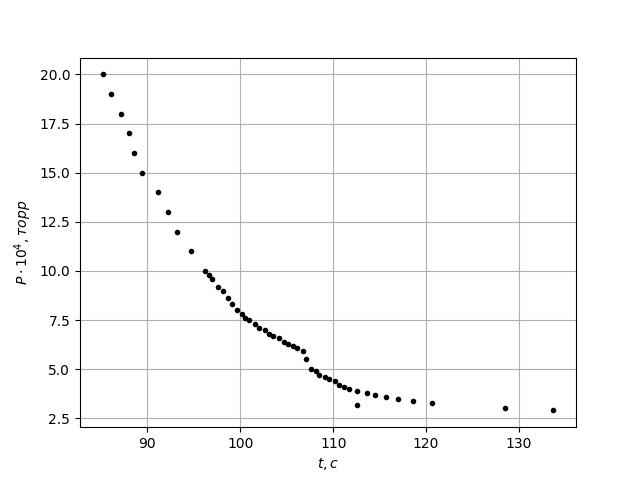
\includegraphics[scale=1]{график улучшения.png}}
\caption{\textit{. График улучшения вакуума.}}
\end{figure}

\begin{figure}
\center{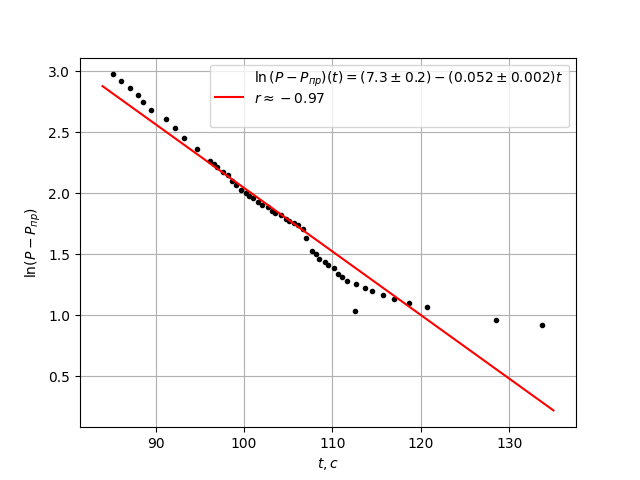
\includegraphics[scale=1]{улучшение логарифм первый вариант}}
\caption{\textit{. Линеаризация графика улучшения вакуума.}}
\end{figure}

\begin{figure}
\center{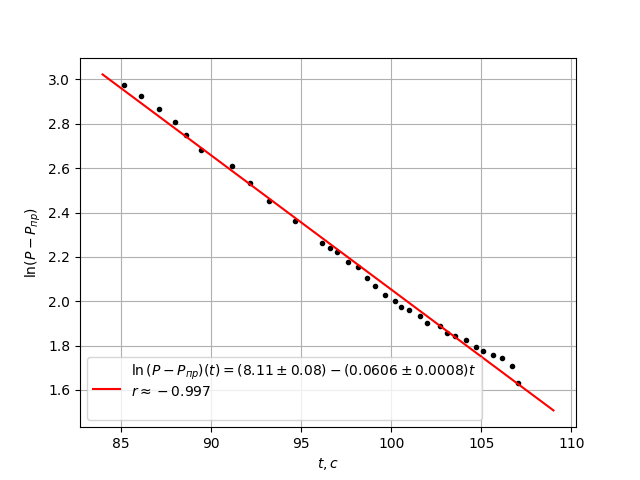
\includegraphics[scale=1]{улучшение логарифм второй вариант}}
\caption{\textit{. Линеаризация графика улучшения вакуума (высокие давления).}}
\end{figure}

\begin{figure}
\center{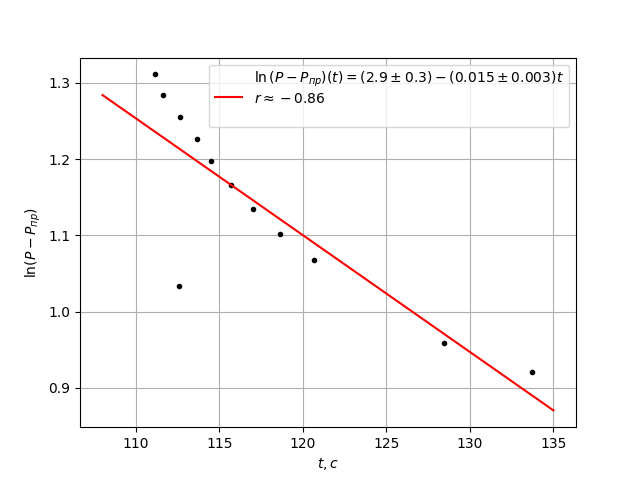
\includegraphics[scale=1]{улучшение логарифм третий вариант}}
\caption{\textit{. Линеаризация графика улучшения вакуума (низкие давления)}}
\end{figure}

\noindent
Значение $W_3$ сильно отличается от остальных, поэтому не будем его учитывать. Тогда, усредняя, получим:
\[W = (0.0735 \pm 0.0016) \ \frac{\text{л}}{\text{с}}\] 

\item[\textbf{10. }] Оценим величину потока газа $Q_{\text{н}}$, поступающего из насоса назад в откачиваемую систему. Из формулы \eqref{pump} и условия, что при ухудшении вакуума $dP/dt = (Q_{\text{д}} + Q_{\text{и}})/V_{vv}$, получим:
\[Q_{\text{н}} = P_{\text{пр}} W - \alpha V_{vv}, \]
где $\alpha = dP/dt$ определяется из анализа зависимости $P(t)$ при ухудшении вакуума по МНК. Получим:
\[\alpha = (2.81 \pm 0.05) \cdot 10^{-6} \ \frac{\text{торр}}{\text{с}} \]
\[Q_{\text{н}} = (1.18 \pm 0.12) \cdot 10^{-6} \ \frac{\text{торр} \cdot \text{л}}{\text{с}} \]

\begin{figure}
\center{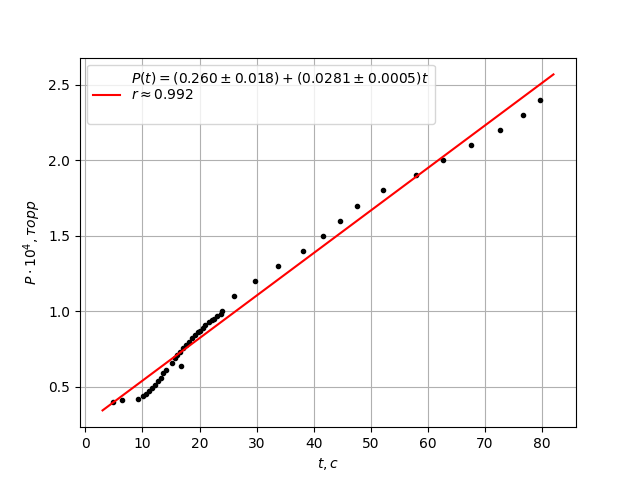
\includegraphics[scale=1]{ухудшение.png}}
\caption{\textit{. График ухудшения вакуума}}
\end{figure}


\end{itemize}
\end{document}